\chapter{Deformation studies of a ladder under the test beam}

  The first full-scale prototype which embeds twelve sensors glued on a copper flex-cable and a 8 \% density \gls{SiC} foam was tested in November 2011 at CERN-SPS facility with a pions beam of 120 GeV.
  The motivations to perform such a test in real conditions are to, firstly, make sure that the ladder is working properly.
  Secondly, to verify the response homogeneity of each sensor.
  Finally, it has to prove the benefits of a double sided measurement.
  This chapter does not aim to present fully the test beam campaign and all the results, but to focus on a specific study of the ladder's deformation observed during the alignment procedure.
  More results about this test beam is presented in Loic Cousin's thesis\cite{cousin}.
  This chapter will present the test beam facility, as well as the experimental set-up.
  The alignment procedure is explained and some results for the ladder positioned in a normal incidence, as well as the ladder titled in one direction are discussed.
  The second part of the sensor will focus on the deviation observed during the alignment and will discuss a method to overcome these deformations.
  Finally, the benefits of double-sided measurements will be introduced.
  
  \minitoc

  \section{Test beam of the full complete PLUME ladder at CERN}

    \subsection{Test beam facility and beam test set-up}

    The test beam was performed at CERN-SPS in the North hall on the H6 beam line.
    Negative pions with an energy of 120 GeV were used.
    The spill structure is 9.6 s with a dead time of 45.6 s. 
    The bench set-up is composed of a telescope made of four standard MIMOSA-26 sensors, thinned down to 120 $\mu\text{m}$ and used as reference planes.
    The telescope is made of two arms, with a distance between the two sensors of the arm of 5 mm.
    The reference planes are stabilised to a temperature of 15 degrees Celsius and a threshold at 8 sigma S/N cut was applied.
    In the middle of the two arms, the PLUME ladder is placed and for the next of the chapter it is denominated as the \gls{DUT}.
    The bench has also $7 \times 7$ scintillators used for triggering the data.
    Most of the runs were taken with a trigger frequency between 2 and 8 kHz, except for two days where the frequency was oscillating between 1 and 1.3 kHz.
    The acquisition system is limited to eight inputs and four inputs are used by the telescope.
    Thus, only four sensors of the \gls{DUT} were connected to the acquisition, two on each side.
    The temperature of the \gls{DUT} was stabilised thanks to air flow cooling system, provided by a fan.

    %The bench set-up is composed of 4 standards 120 $\mu\text{m}$ thinned MIMOSA-26 used as telescope planes, the PLUME ladder, called here \gls{DUT} and a $7 \times 7 \text{mm}^2$ used for triggering. 
    %The reference planes are at 8 sigma S/N cut and stabilized to a temperature of 15 degrees Celsius.
   % The telescope is made of two arms, on each side of the \gls{DUT} and the distance between two sensors of the same arm is 5 mm.
    %Nonetheless, for one experimentation, the telescope was set-up differently, as discussed later.
    %Most of the runs were taken with a trigger frequency between 2 and 8 kHz except for two days on which it was between 1 and 1.3 kHz.
    %As the acquisition system is limited to eight inputs and the set-up has four reference planes, only four sensors of the \gls{DUT} were connected, two on each side.
    %Nevertheless, due to the size of the scintillator, the acquisition of sensors outside the beam is not mandatory. 
    %Thus, it reduces the data band-with.
    %Two different air flow speeds were used: 3 $\text{m.s}^{-1}$ and 6 $\text{m.s}^{-1}$. 

    \subsection{Cartesian coordinate systems}

    Although the sensors have their own ID to distinguish them during the analysis, the position of each plane has to be known exactly.
    Two Cartesian coordinate systems are then defined.
    The first one is the global one and is determined by the position of each sensors of the telescope.
    The notation used for this coordinate system is $(x,y,z)$.
    The $x$-axis corresponds to the horizontal direction, the $y$-axis is the vertical direction and the $z$-axis is along the beam direction.
    The origin $(0,0,0)$ is of the system is defined with respect to the center of the two reference planes arms.
    The second coordinate system is the local one and is determined for a single sensor.
    To differentiate this reference the $(u,v,w)$ notation is used.
    The $u$-axis corresponds to the pixel rows, the $v$-axis is along the pixel columns and the $w$-axis is perpendicular to the matrix.
    The origin of the local system is the center of the pixel matrix.
    The figure~\ref{fig:labCoordinates} summarises the definition of the two coordinate systems.

    \begin{figure}
      \centering
      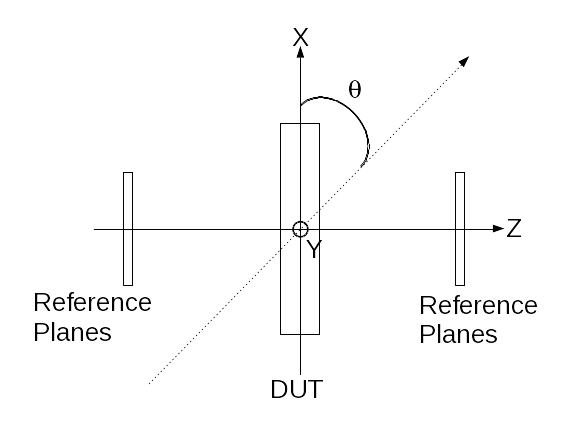
\includegraphics[width = 0.7\textwidth]{Pictures/deformation/lab_frame.png}
      \caption{Drawing of the laboratory coordinates.}
      \label{fig:labCoordinates}
    \end{figure}

    \subsection{Measurements}

    The prototype validation was done under several conditions.
    Firstly, three different geometric configurations were used.
    On the first one presented on the figure~\ref{fig:tbNormal}, the \gls{DUT} is parallel to the telescope planes and the beam is hitting the device in a normal incidence.
    The \gls{DUT} is placed in between the two arms, with the middle in a center of the foam.
    For the second configuration, as shown on the figure~\ref{fig:tilt36}, the distance between the telescope planes are the same, but the \gls{DUT} is tilted between 28 and 40 degrees along the $y$-axis.
    Runs with a larger angle (60 degrees) were done.
    Due to the PLUME box's size, the cabling for the acquisition, the air cooling system and the design of the telescope stage, limiting the spacing between the two arms, the \gls{DUT} was placed behind the two arms, as presented on the figure~\ref{fig:tilt60}.
    For both configurations, different parameters were modified.
    The thresholds was set to 5 and 6 mV, different sensors were aimed and the air flow speed was set to 3 $\text{m.s}^{-1}$ and 6 $\text{m.s}^{-1}$.

    \begin{figure}[!h]
      \centering
      \begin{subfigure}[t]{0.9\textwidth}
        \centering
        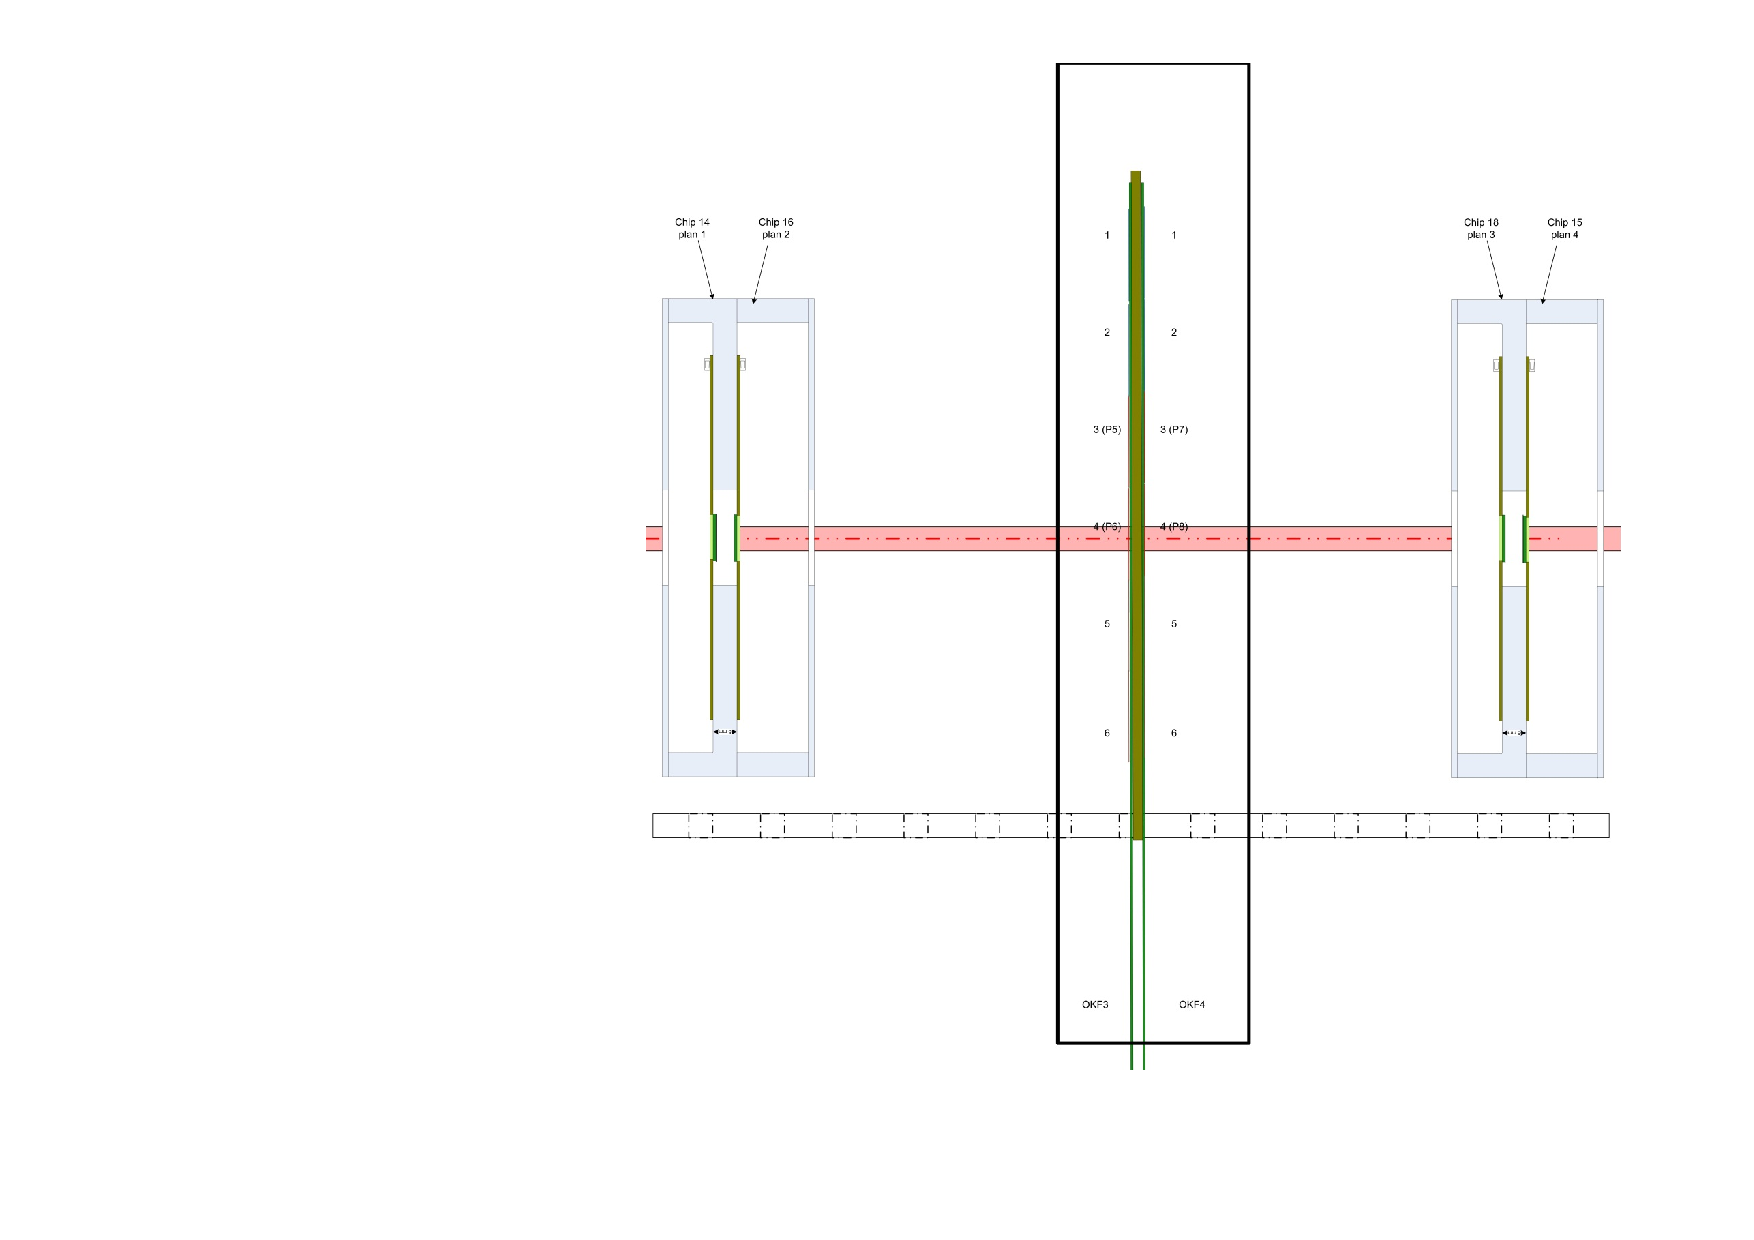
\includegraphics[width = 0.5 \textwidth]{Pictures/deformation/tb_cern_11_sketch_normal.pdf}
        \caption{Set-up for the PLUME ladder in normal incidence with respect to the beam direction.}
        \label{fig:tbNormal}
      \end{subfigure}

      \begin{subfigure}[t]{0.45\textwidth}
        \centering
        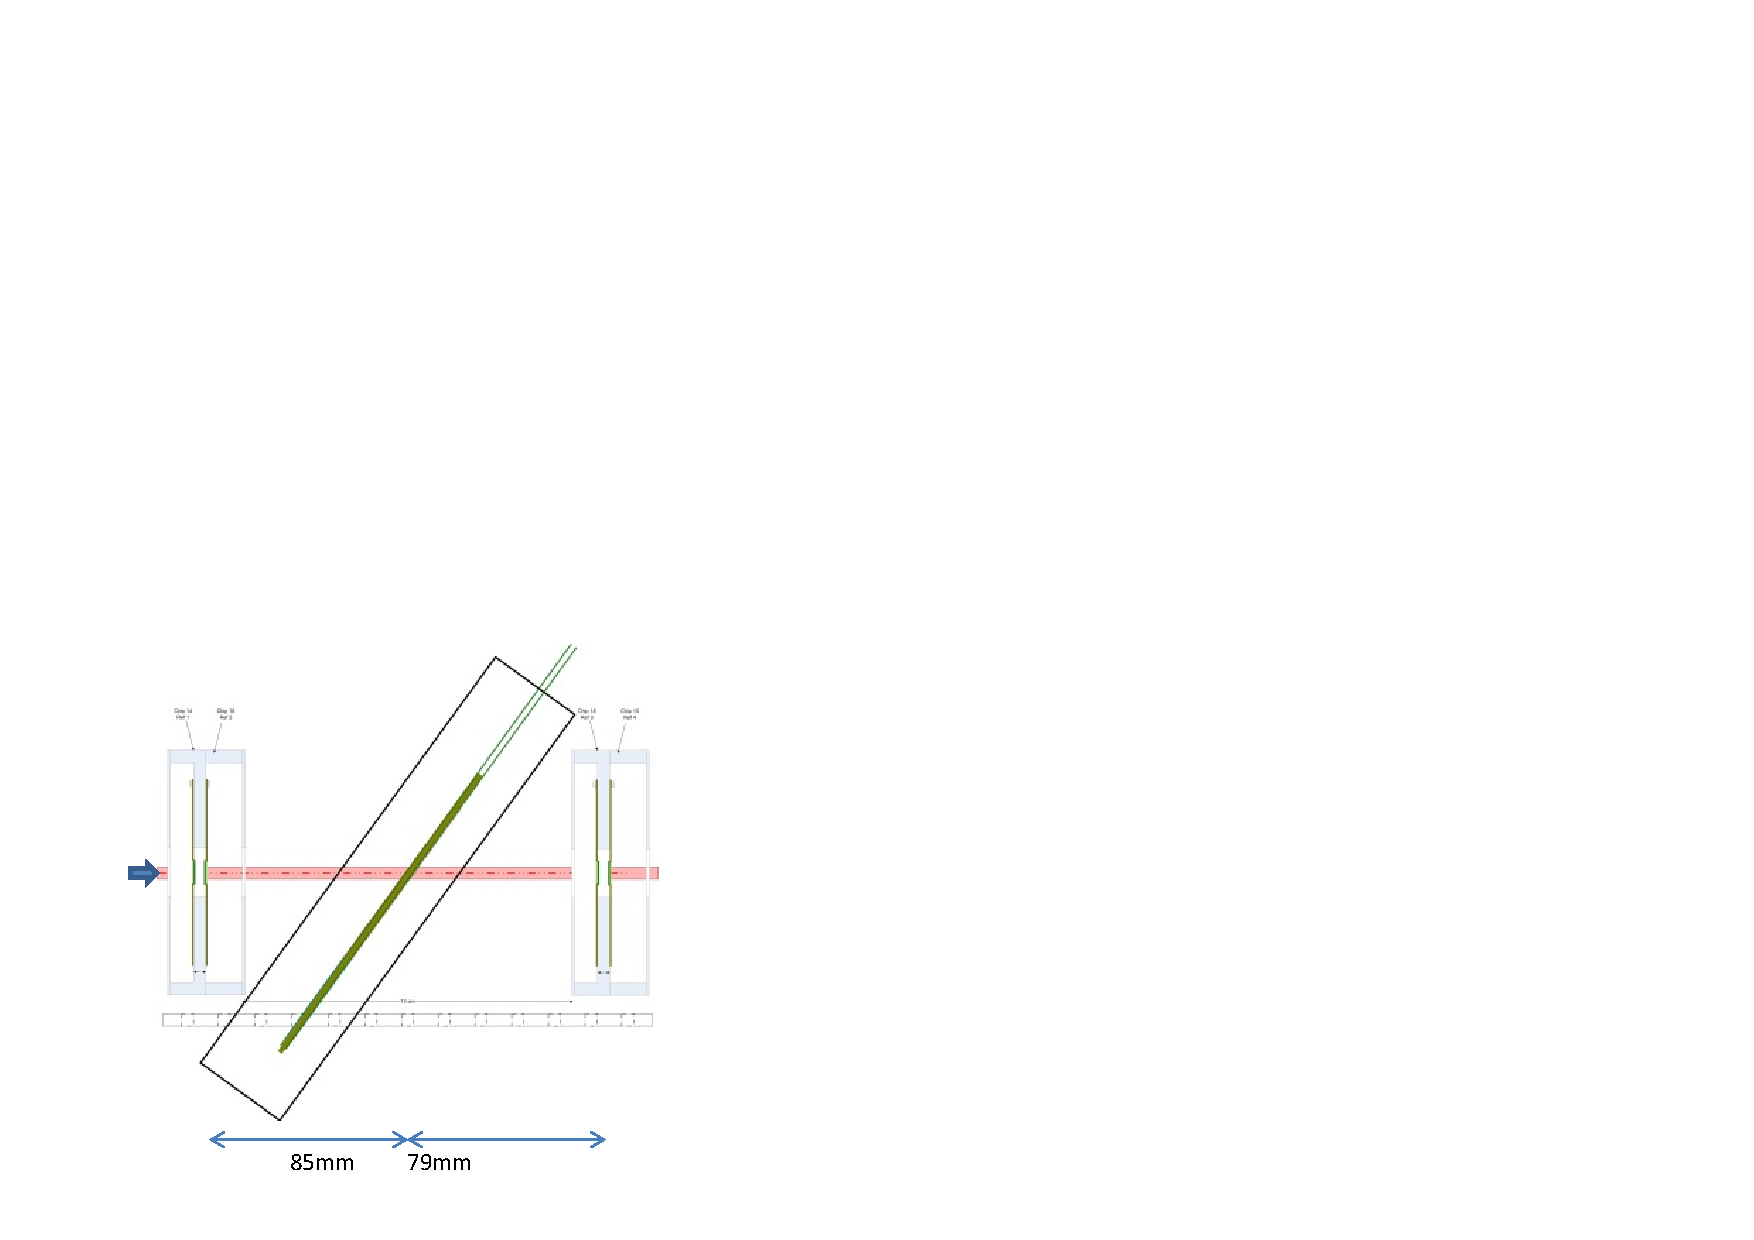
\includegraphics[width=0.8\textwidth]{Pictures/deformation/tb_cern_11_sketch_tilted.pdf}
        \caption{Configuration for an angle between 28 and 40 degrees.}
        \label{fig:tilt36}
      \end{subfigure}
      ~%\quad
       %add desired spacing between images, e. g. ~, \quad, \qquad, \hfill etc. 
        %(or a blank line to force the subfigure onto a new line)
      \begin{subfigure}[t]{0.45\textwidth}
        \centering
        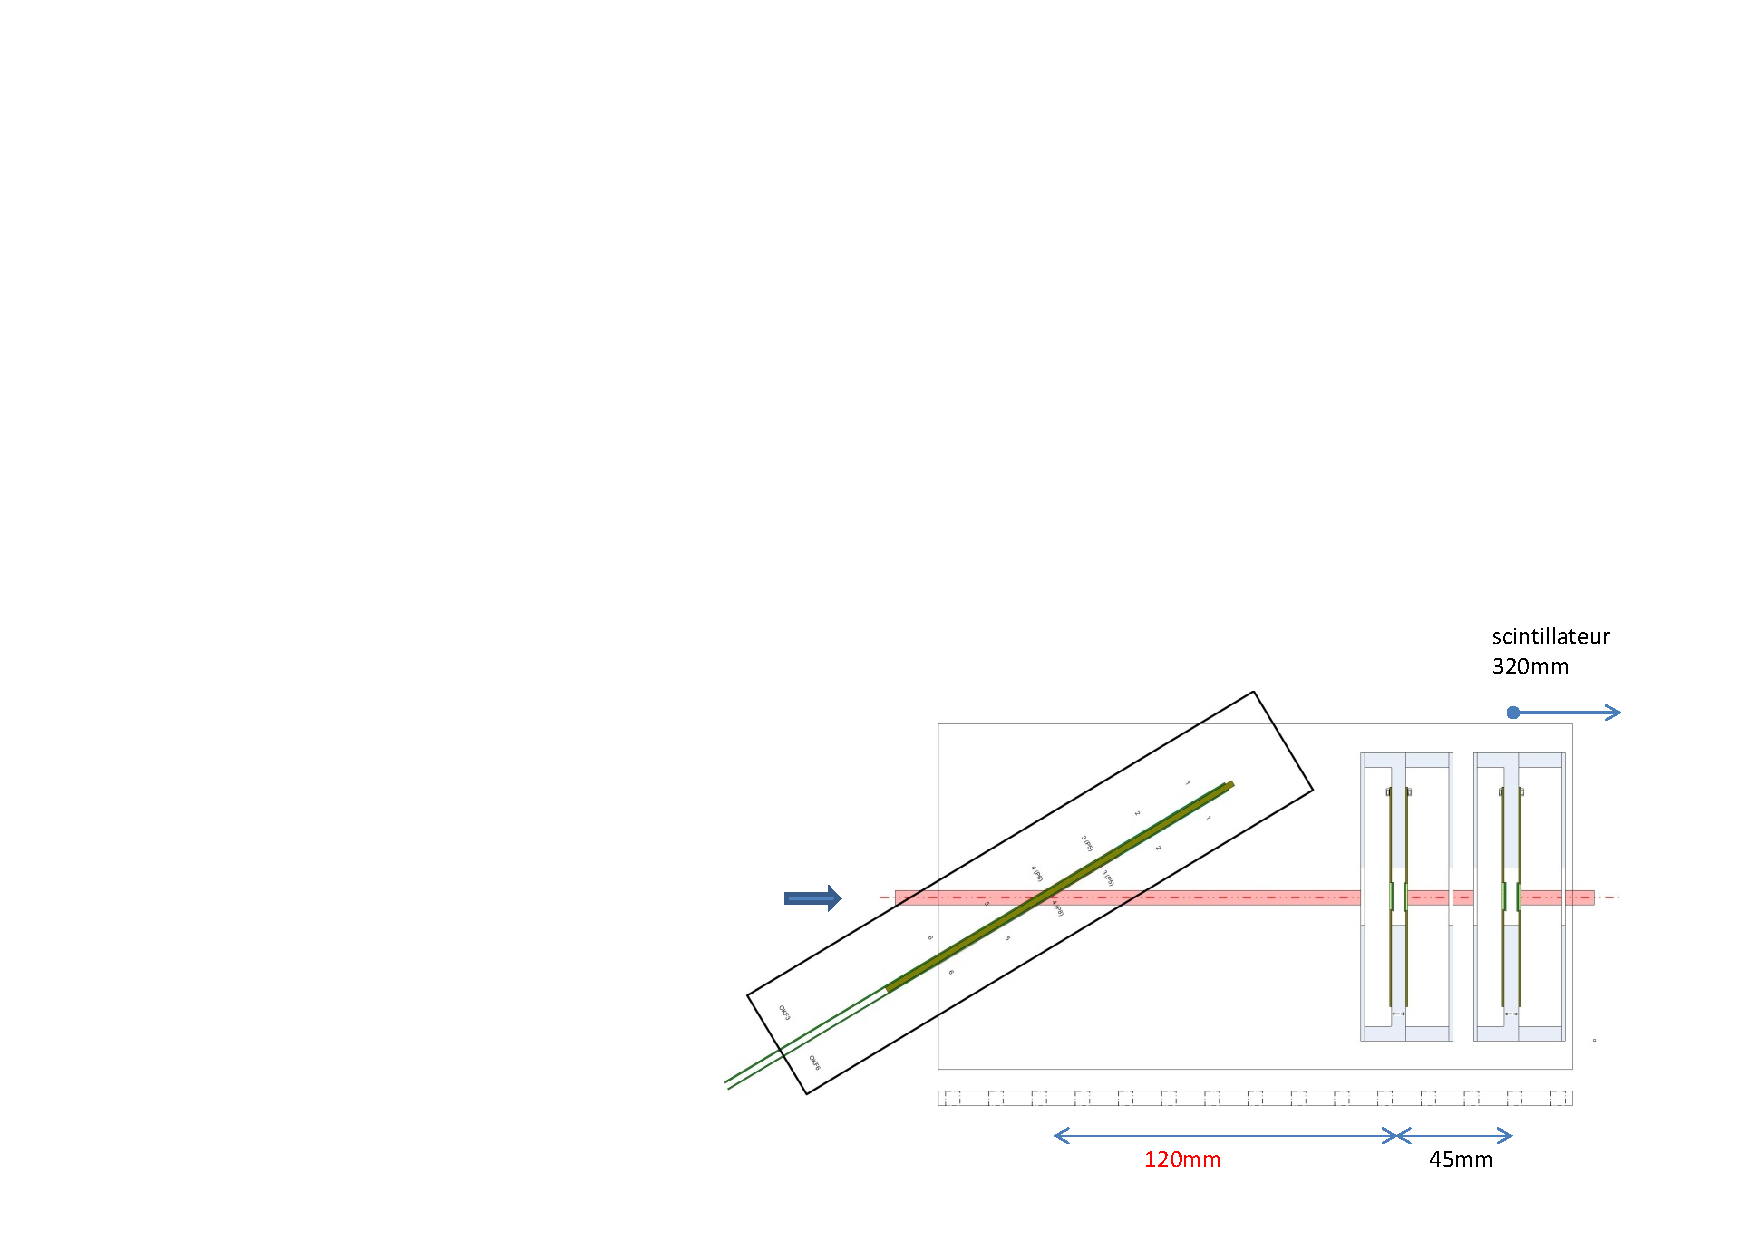
\includegraphics[width=0.95\textwidth]{Pictures/deformation/tb_cern_11_sketch_tilted120mm.pdf}
        \caption{Configuration for an angle of 60 degrees.}
        \label{fig:tilt60}
      \end{subfigure}
      \caption{Top view sketches of the test beam configuration for different ladder positions.}
      \label{fig:tilt}
    \end{figure}   

    The analysis and the results shown in the following sections were done thanks to \gls{TAF}, the analysis software developed by the IPHC.

  \section{Spatial resolution studies}
   
    One of the measurement performed during the analysis is to determine the pointing resolution of the ladder.
    The sensors used are well-known and they should have a pointing resolution similar to the one expected, regardless the mechanical structure.
    Any deviations might point out an impact of the mechanical structure on the whole system.
    To get the better understanding, different running conditions were performed: different air flow speed to cool the ladder, different threshold levels and different orientation on of the ladder with respect to the beam.

    \subsection{Normal incidence track}

    Only the hit position is provided by the each sensor.
    To perform an analysis, the telescope planes have to be aligned each other to form tracks from the hit information.
    A track correspond to the path of a particle through the system.
    Thanks to this information, the tracks are then compared to the hit position on the \gls{DUT} to give some information, such as the detection efficiency (the ratio of tracks matched to hits on the \gls{DUT}), the spatial resolution (minimum distance to distinguish two incoming tracks).

    The alignment procedure is done in two steps: firstly the telescope planes are aligned and then the \gls{DUT} is aligned with respect to the information provided by the reference planes. 
    Although the position of each sensors is measured during in the test beam with a precision of the millimeter, for the analysis, a precision of the micron level has to be achieved.
    During the analysis, three degrees of freedom were taken into account for the alignment: two translations for the $x$ and $y$-axes and one rotation around the $z$-axis.
    The $z$ position is here fixed with respect to the measurement performed during the test beam campaign.

      \subsubsection{Alignment procedure}

      Firstly, the data are processed to extract the signal and the hit information.
      The hit is defined as each pixel having a signal above the discriminator thresholds.
      The pixels fired are grouped into cluster.
      As the sensors used have a binary output, no information on the seed pixel is provided.
      Thus, the hit position is obtained from a center of gravity calculation.

      Secondly, the tracks are reconstructed from the hit position.
      One plane is the origin of the global coordinate system and it is generally the first reference plan hit by the beam.
      The track candidates are built perpendicular from the hit found in this first sensor and then extrapolated to the next planes.
      The alignment is an iterative procedure that consists to minimise the residual, or the distance between the track extrapolated to the closest hit on the sensor.
      For example, a track is built from the first reference plane and extrapolated to the last reference plane.
      The residual is minimised and then, a track is defined as straight line connecting one hit on the first plane to a hit on the last plane.
      The sensors in the middle are aligned with respect to this track candidate.
      After the telescope alignment, a track candidate is dismissed if it is made of less than four hits or if the $\chi^2$ fit is greater than a fixed value determined by the user. 

      For the alignment, two assumptions are defined. 
      The telescope planes are parallel each other.
      Thus the alignment consists of a translation along $x$ and $y$ and a rotation around the $z$-axis.
      As the test beam was performed without a magnetic field and pions of 120 GeV were used, the Coulomb multiple scattering is neglected.
      So, the tracks are perpendicular to the detectors and the alignment is not sensitive to the $z$ position.
      A precision of the millimeter level for the position does not have a huge impact on the alignment.

      \subsubsection{Alignment of the DUT}

      When the telescope alignment is done, the reference tracks reconstructed by the reference planes are used to align the \gls{DUT}.
      Its $z$ position is fixed, nonetheless, two degrees for freedom are added: the rotations along the $x$ and $y$-axes, plus the three other degrees of freedom defined above.

      \begin{figure}
        %\centering
        \missingfigure{Track-hit residual as a function of the hit position (normal incidence)}
      \end{figure}



    \subsection{Ladder tilted in one direction}

      The same alignment procedure, as presented above, was applied for runs where the ladder was tilted with respect to the beam direction, as shown on the figure~\ref{fig:tilt}.
      Nevertheless, the alignment is more complicated.
      
      \begin{figure}
        %\centering
        \missingfigure{Track-hit residual as a function of the hit position (tilt)}
      \end{figure}
    
      \subsubsection{Origin of the deviations}

      \begin{figure}
        %\centering
        \missingfigure{Explanation of deviations}
      \end{figure}

      \subsubsection{Algorithm to estimate the deformations}

      \begin{figure}
        %\centering
        \missingfigure{Residual after correction}
      \end{figure}
    
  \section{Benefits of double-sided measurement}

  %\todo{REF Loic thesis for TB@CERN results}
